\section{DNA Thermodynamics}

\begin{figure}[ht]
  \begin{centering}
  \adjustbox{minipage=1.3em,valign=t}{\subcaption{}\label{sfig:testa}}%
  \hspace{-0.3cm}
  \begin{subfigure}[t]{\dimexpr.15\linewidth-1.3em\relax}
  \centering
  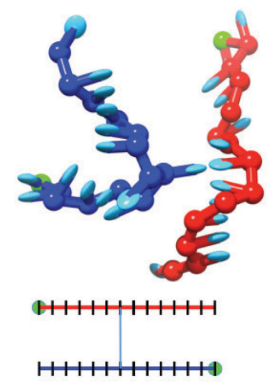
\includegraphics[width=1.06\linewidth,valign=t]{Figures/hybridDiag1.png}
  \end{subfigure}%
  \adjustbox{minipage=1.3em,valign=t}{\subcaption{}\label{sfig:testa}}%
  \hspace{-0.35cm}
  \begin{subfigure}[t]{\dimexpr.15\linewidth-1.3em\relax}
  \centering
  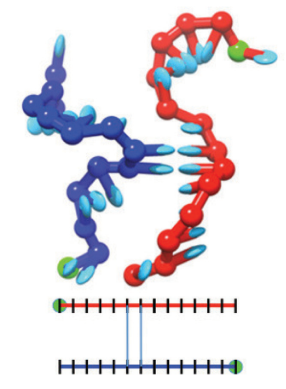
\includegraphics[width=1.09\linewidth,valign=t]{Figures/hybridDiag2.png}
  \end{subfigure}%
  \adjustbox{minipage=1.3em,valign=t}{\subcaption{}\label{sfig:testb}}%
  \hspace{-0.28cm}
  \begin{subfigure}[t]{\dimexpr.15\linewidth-1.3em\relax}
  \centering
  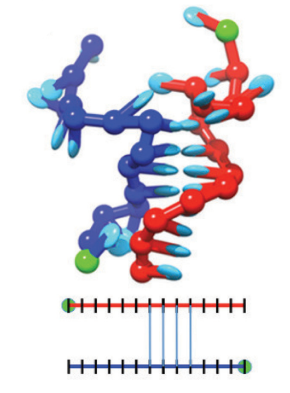
\includegraphics[width=1.1\linewidth,valign=t]{Figures/hybridDiag3.png}
  \end{subfigure}
  \adjustbox{minipage=1.3em,valign=t}{\subcaption{}\label{sfig:testa}}%
  \hspace{-0.21cm}
  \begin{subfigure}[t]{\dimexpr.15\linewidth-1.3em\relax}
  \centering
  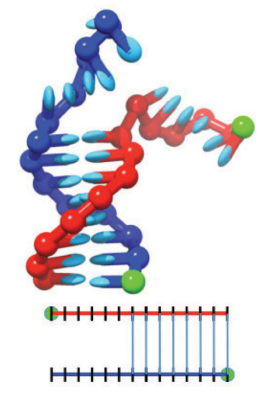
\includegraphics[width=.98\linewidth,valign=t]{Figures/hybridDiag4.png}
  \end{subfigure}%
  \adjustbox{minipage=1.3em,valign=t}{\subcaption{}\label{sfig:testa}}%
  \hspace{-0.38cm}
  \begin{subfigure}[t]{\dimexpr.15\linewidth-1.3em\relax}
  \centering
  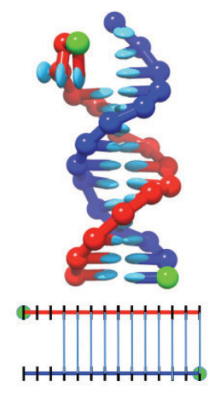
\includegraphics[width=.8\linewidth,valign=t]{Figures/hybridDiag5.png}
  \end{subfigure}
  \adjustbox{minipage=1.3em,valign=t}{\subcaption{}\label{sfig:testb}}%
  \hspace{-0.5cm}
  \begin{subfigure}[t]{\dimexpr.2\linewidth-1.3em\relax}
  \centering
  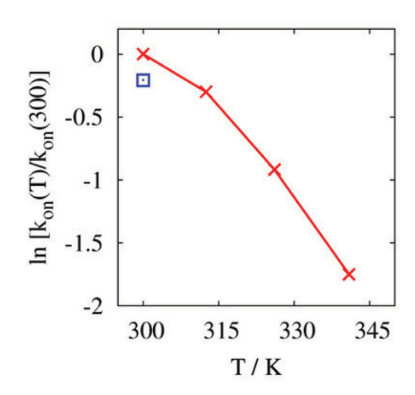
\includegraphics[width=1.5\linewidth,valign=t]{Figures/hybridDiag6.png}
  \end{subfigure}
  \caption{This is a figure [.]}
  \label{fig:test}
  \end{centering}

\end{figure}


hybridisation

Intiating strand displacement incurs a thermodynamic penalthy
(making is difficult to simulate). initial contacts often dissociate, despite
non-negligible attractive inter- actions, because their configurations are not conducive
to full duplex formation

to obtain good statistics FFS is needed. one of the main reasons is many different
transition paths that exist. Different hybridisation path ways are called Inchworm and
pseudoknot often occur in repetitive sequences. the system does not possess a single,
well-defined ‘transition state’ but a complex ensemble of transition pathways


‘fraying’ to describe the disruption of base pairs at the end of a duplex; if all base
pairs fray, the duplex melts or dissociates.

‘zippering’ refers to when a new base pair forms at the end of an existing duplex

Watson–Crick complementary reduces free energy

-----------------------------------------------------------------------------------------
Toehold mediated strand displacement.

strand displacement increases number of hybridised base pairs, fully Watson–Crick
complementary -> descreasing the overall free energy of the system. Overall, displacement
is thermodynamically driven forward by the net gain in base pairs due to the toehold


Once the toehold has bound, there are two possibilities: (i) the toehold base pair could
dissociate, leading to the dissoci- ation of the invader or (ii) the nearest base pair of
the substrate-incumbent complex could fray, allowing the invader to compete to replace
that base pair and complete the first step of branch migration.

as may seem reasonable, that the rate at which either base pair frays is similar, process
(ii) should be approximately half as fast as process (i).  strand displacement kinetics
depends on toehold length.  Intiating strand displacement incurs a thermodynamic penalthy
(making is difficult to simulate).

This is because, once the substrate- incumbent base pair frays, there is a 50% chance of
the invader replacing the frayed base pair, and a 50% chance of returning to the initial
step.

Therefore, the probability of successfully completing the remaining steps ofbranch
migration before going back to the toehold-only- bound state is 1/20, from the gambler’s
ruin analysis

model branch migration at a more detailed level. we analyze a 1D (single-pathway) model
of toehold-mediated strand displacement called the intuitive energy landscape (IEL) model
-> refer to graph on image.


\begin{figure}[ht]
\begin{center}
  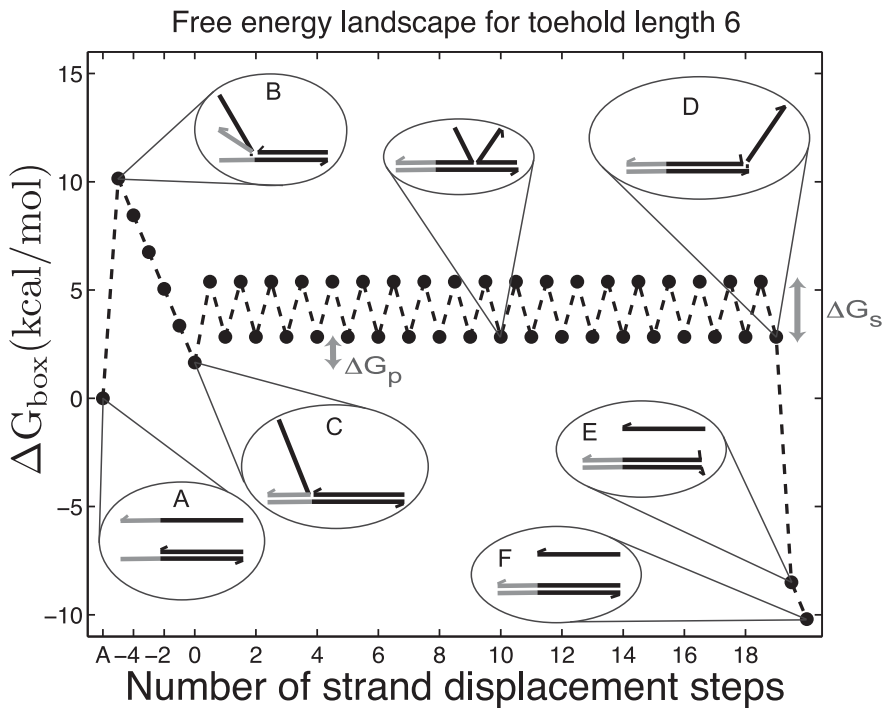
\includegraphics[width=0.5\textwidth]{Figures/ToeholdDiagram.png}
  \caption{write caption[.]}
\end{center}
\end{figure}


